\documentclass[11pt]{amsart}

\usepackage{mathptmx}
\usepackage{a4wide}
\usepackage{graphicx}

\begin{document}

\section{Classification results}

\begin{center}
  \begin{tabular}[c]{llll}
    file
    & team
    & is matroid?
    & execution time
    \\\hline
    \texttt{1716.bases}
    & Team Bearland
    & yes
    & 0.33 s
    \\
    & other-awesome-team-name
    & yes/no
    & [seconds]
    \\\hline
      \texttt{252.bases}
    & Team Bearland
    & yes
    & 0.007 s
    \\\hline
      \texttt{3432.bases}
    & Team Bearland
    & yes
    & 1.276 s
    \\\hline
      \texttt{4092.bases}
    & Team Bearland
    & no
    & 0.019 s
    \\\hline
      \texttt{417.bases}
    & Team Bearland
    & no
    & 0.002 s
    \\\hline
      \texttt{462.bases}
    & Team Bearland
    & yes
    & 0.021 s
    \\\hline
      \texttt{4639.bases}
    & Team Bearland
    & no
    & 0.397 s
    \\\hline
    \texttt{6435.bases}
    & Team Bearland
    & yes
    & 4.506 s
    \\\hline
    \texttt{924.bases}
    & Team Bearland
    & yes
    & 0.088 s
    \\\hline
    \texttt{definetely-bases.txt}
    & A-Team-Has-No-Name
    & yes
    & 0.00024 s
    \\\hline
    \texttt{not-bases-1.txt}
    & A-Team-Has-No-Name
    & no
    & 0.00028 s
    \\\hline
    \texttt{not-bases-2.txt}
    & A-Team-Has-No-Name
    & no
    & 0.000006 s
    \\\hline
    \texttt{252.bases}
    & A-Team-Has-No-Name
    & yes
    & 0.597 s
    \\\hline
    \texttt{417.bases}
    & A-Team-Has-No-Name
    & no
    & 0.219 s
    \\\hline
    \texttt{462.bases}
    & A-Team-Has-No-Name
    & yes
    & 2.373 s
    \\\hline
    \texttt{924.bases}
    & A-Team-Has-No-Name
    & yes
    & 11.81 s
    \\\hline
    \texttt{1716.bases}
    & A-Team-Has-No-Name
    & yes
    & 46.30 s
    \\\hline
    \texttt{3432.bases}
    & A-Team-Has-No-Name
    & yes
    & 220.7 s
    \\\hline
    \texttt{4092.bases}
    & A-Team-Has-No-Name
    & no
    & 2.50 s
    \\\hline
    \texttt{4639.bases}
    & A-Team-Has-No-Name
    & no
    & 57.37 s
    \\\hline
    \texttt{6435.bases}
    & A-Team-Has-No-Name
    & yes
    & 917.4 s
    \\\hline    
  \end{tabular}
\end{center}

\section{Execution times}

\subsection{Team Bearland}

We implemented a mask-based algorithm.
Each mask $m$ represents a set.
The $i$-th bit of the mask is set to 1 iff $i$ belongs to the set.
We can easily, and in a fast manner, access each position shifting bits, and unions, intersections and complements are solved using bitwise OR, AND, NOT, and XOR operators.
The code implemented in \textsc{Python3}, albeit leveraging the same principle, implements the masking operations differently.
 
In both cases, the complexity is the same. We take advantage of the fact that all values in all inputs are integers between $0$ and $r - 1 = 19$. In every case, we build the masks in $\mathcal{O}(\sum_{B \in \mathcal{B}} |B|) = \mathcal{O}(r|\mathcal{B}|)$ time. Then, for each pair $(B_1, B_2) \in \mathcal{B} \times \mathcal{B}$, we check that the exchange conditions by taking all $\mathcal{O}(r)$ values of $x \in B_1$, and checking if the condition holds for each of the $\mathcal{O}(r)$ possible values of $y \in B_2$, and we also check that $x \in B_1 \setminus B_2$ and $y \in B_2 \setminus B_1$ in $\mathcal{O}(r^2)$ time. Finally, we check that the mask for $B_1 \setminus \{x\} \cup \{y\}$ belongs to the set of masks in $\mathcal{O}(\log(|\mathcal{B}|))$ time. Therefore, the total complexity is $\mathcal{O}(r |\mathcal{B}|) + \mathcal{O}(r^2 |\mathcal{B}|^2| \log(|\mathcal{B}|)) =  \mathcal{O}(r^2 |\mathcal{B}|^2| \log(|\mathcal{B}|))$.

Figure~\ref{fig:team-bearland-times} summarizes the execution times for both programming languages.
Note that we re-ordered the results to plot them in a, more or less, increasing fashion. 
\begin{figure}[h!]
    \centering
    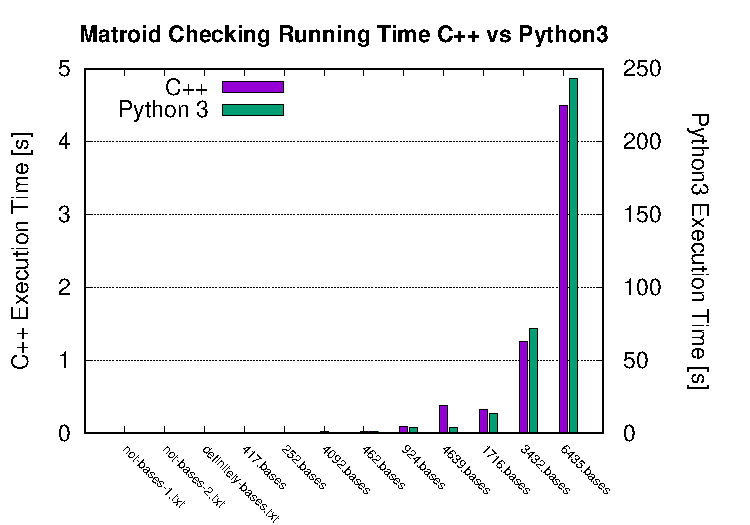
\includegraphics[width=.7\textwidth]{./team-berland/exec_time.pdf}
    \caption{Execution time of the two different implementations in increasing order.\label{fig:team-bearland-times}}
\end{figure}
The results were to be expected, the compiled, performance-oriented, \textsc{C++} implementation outruns the \textsc{Python3} one by two orders of magnitude.
However, we do observe that the behaviour, the pattern described by execution times as we increase the load (\textit{i.e.} the complexity) is the same for both algorithms.
This is a great example not to underestimate the constants affecting our expected running time, usually disregarded by complexity theory and big $\mathcal{O}$ notation.
%Under our point of view, each programming language has it's 

\subsection{A-team-has-no-name}

1)Our code can process all the files, but the Haskell version takes 11 thousand seconds for the largest file and the python best algorithm takes 917 seconds which is still a lot.

2)If n is the number of elements in $\mathcal{B}$ and m the max number of elements in any of the elements of $\mathcal{B}$, our first python code runs in $\mathcal{O}(n^3)*\mathcal{O}(m^4)$.
We could reduce the complexity concerning m, but as in almost any case we can find m is going to be a constant amount compared to n, we have not worried a lot about it as the complexity for those kinds of general examples is actually $\mathcal{O}(n^3)$.
We tried to reduce this complexity by trying to check relations between the elements in B but at first we ended up making the complexity worse, and then when improved we returned back to $\mathcal{O}(n^3)$ but reducing the running time to a 60\%-70\% of the original one for the files we processed.

Haskell code runs equally in $\mathcal{O}(n^3)$.

For the second python code we thought about using a biyection between sets and integer number so that we could order the list of sets and check if $B_1$ is in the list in logarithmic time.
This was done by assigning every set the sum of 2 powered to every of the elements in the set. 
This assumes that we are using integers for each set in the matroid and that there are not a lot of elements in total. If there were other elements that were not integers we could do a bijection between the elements and $\mathbb{Z}$ so we could apply this method.
This allows us to avoid the last loop by using a binary search in the ordered set of values of each element in the matroid, reducing the complexity to $\mathcal{O}(n^3)*\log(n)$. 
If m was big we expect this algorithm to be worse than the first one, so it is input sensitive. 

It is also worth mention that both of the python algorithm will stop as soon as they find a $B_1$ that does not verify the condition, and that is why 4096.bases files or similar get checked so quickly.


\subsection{other-awesome-team-name}

another plot here

\end{document}
